\chapter{基于南极的天文数据观测与处理} \label{chapter:obs_red}

\section{南极天文背景} \label{sec:antarticabg}

搜索系外行星需要长时间基线和高精度的天文观测,然而因为地球在做周日自转并且存在大气包层,
因而在地球上很难同时满足这些严苛的观测条件。\S \ref{sec:transit} 中曾提到空间望远镜 CoRoT
\cite{Bargeetal2008CoRoT} 与 $Kepler$\cite{Boruckietal2010},它们花费了昂贵的代价(数十亿
美元)才能得到满足上述观测条件的数据,事实证明它们也取得了令人瞠目的科学成果。而横向对比,
南极台址(Antarctic plateau)作为理想的地面台址可在花费相对较少经费的同时,依然拥有良好的
观测条件 --- 这得归功于此台址以下几点优势:

\begin{enumerate}[leftmargin=1\parindent] 
\item[--] 南极高台地址拥有大陆上最冰冷、干燥\footnote{以绝对水气值来衡量。}的空气(文献\citen{Burton2010} )。此气候条件尤为适合进行光学、红外以及亚毫米波段的天文观测\cite{Lawrence2004}。
\item[--] 南极高台水平高度高,因而空气层厚度薄,大气湍流少,空气状况也更稳定\cite{Bonner2010}。
\item[--] 极夜(Polar nights)为观测提供了长达 3 个月的连续观测条件,这也是对于系外行星探测最重要的优势\cite{Rauer2008}。
\end{enumerate}

\begin{figure}[t]
\centering
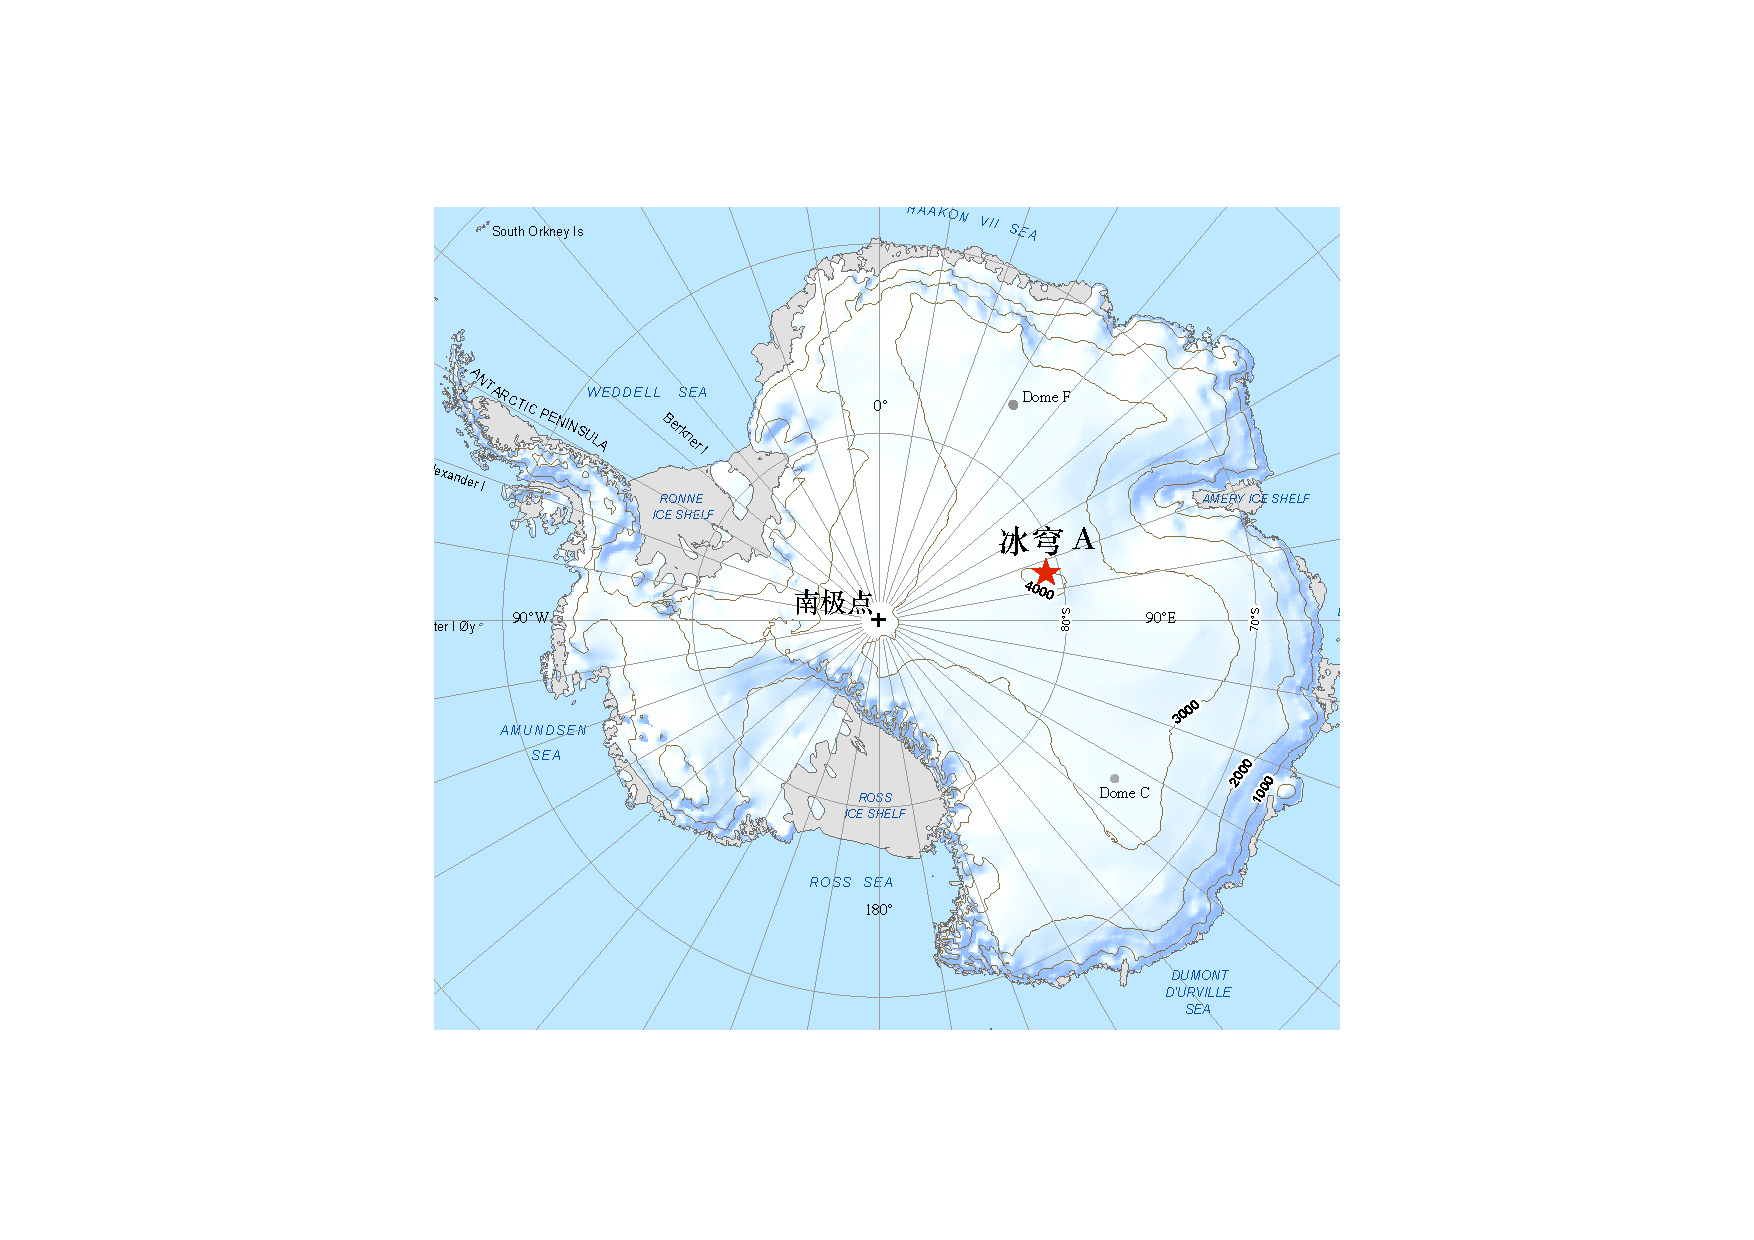
\includegraphics[width=1.0\textwidth]{figures/chapter2/f1_DomeA.pdf}
\caption{南极地理位置图,暗咖啡色曲线表示地形等高线。可以看到 Dome Argus(或称冰穹 A)台址(中国,以红星标注)位于南极大陆最高点,另外冰穹 C(澳洲) 和 F(日本)分别以灰色圆点表示。此地图版权 Australian Antarctic Division。}
\label{fig:domeasite}
\end{figure}

得益于拥有如此得天独厚的先天条件,南极台址在短短 30 年内就已吸引了大批的天文开拓实验与项目
(南极天文的历史相关细节请查阅综述文献\citen{Indermuehle2005})。Grec 等人于 1980 年开启首个
地处南极的光学实验\cite{Grec1980}。随后一大批天文学成果相继涌现\cite{Burton2010},以高精度测光
科学为例:ASTEP(Antarctic Search for Transiting Extrasolar Planets)项目先后于 Dome C 观测台址
捕捉到 WASP-19 b 次掩食的证据\cite{Abe2013STEP},并对该台址在凌星法探测系外行星领域的可行
性作出测试\cite{Crouzet2010}。

Dome A(位于昆仑站附近,坐标 $80^{\circ}37'$ S、$77^{\circ}53'$ E,如图 \ref{fig:domeasite})作为
南极大陆最高的台址(海拔高度 4093m)在南极天文领域有着特殊的地位。Saunders 在比较过云层覆
盖率、空气对流层厚度和视宁度(seeing)后,指出 Dome A 也许是地面潜在的最佳天文观测台址(文
献\citen{Saunders2009})。中国南极天文中心也于 2008 年成功将中国之星小望远镜阵(Chinese 
Small Telescope ARray,简称 CSTAR)成功安装就位于冰穹 A 台址。在极地冰寒的环境下需要克服许多
的障碍\footnote{关于南极天文科考支撑平台,请参见网址 \url{http://www.ccaa.pmo.cas.cn/njtwt/201312/t20131203_144501.html}。},
CSTAR 经过了一代人的奋斗,也取得了丰硕的成果,本文将于 \S \ref{sec:cstar} 中详细介绍如何通过修
正鬼像(ghost image)来提高数据精度。另外 \S \ref{sec:ast3} 将简单描述 AST3(Antarctic Survey 
Telescopes)巡天项目中系外行星搜寻计划的观测策略。


\section{CSTAR 以及其测光数据中的鬼像处理}  \label{sec:cstar}
\subsection{CSTAR 望远镜光学设计和预数据处理}  \label{sec:cstardesign}
作为 PLATO 平台\cite{Lawrence2009,Yang2009}下一台子设备,CSTAR 望远镜由南京天文光学技术研
究所(Nanjing Institute of Astronomical Optics \& Technology,即 NIAOT)承担设计工作。CSTAR 阵
列由 $2\times2$ 共四面施密特卡式(Schmidt-Cassegrain)望远镜组成,每面镜子大小 145 mm 口径:
其中三面拥有与斯隆数字化巡天类似的 $g,\,r,\,i$  宽带滤镜,第四面无滤镜。望远镜被设计固定于地
表,因而采用指向天顶附近南天极天区的凝视观测模式,考虑此做法也是因为这样更有利于研究天文
变源。CSTAR 成像后端匹配了 Andor DV435 型号 1k $\times$ 1k 的 CCD,联合望远镜 $4.5^\circ{} 
\times 4.5^\circ{}$ (20 deg$^2$) 的视场(Field Of View,或 FOV)大小,由此可知一个像素(pixel)对应于
天球 15$''$ 的张角\cite{Yuan2008}。图 \ref{fig:cstaroptics} 展示的是 CSTAR 内部光路结构,在已有的 
$i$ 波段数据中,入射镜的表面覆盖了滤光片,且子镜(中间镜)也涂有反射膜,恒星的光线容易在两面
涂层之间反射,从而导致鬼像的产生。

\begin{figure}[t]
\centering
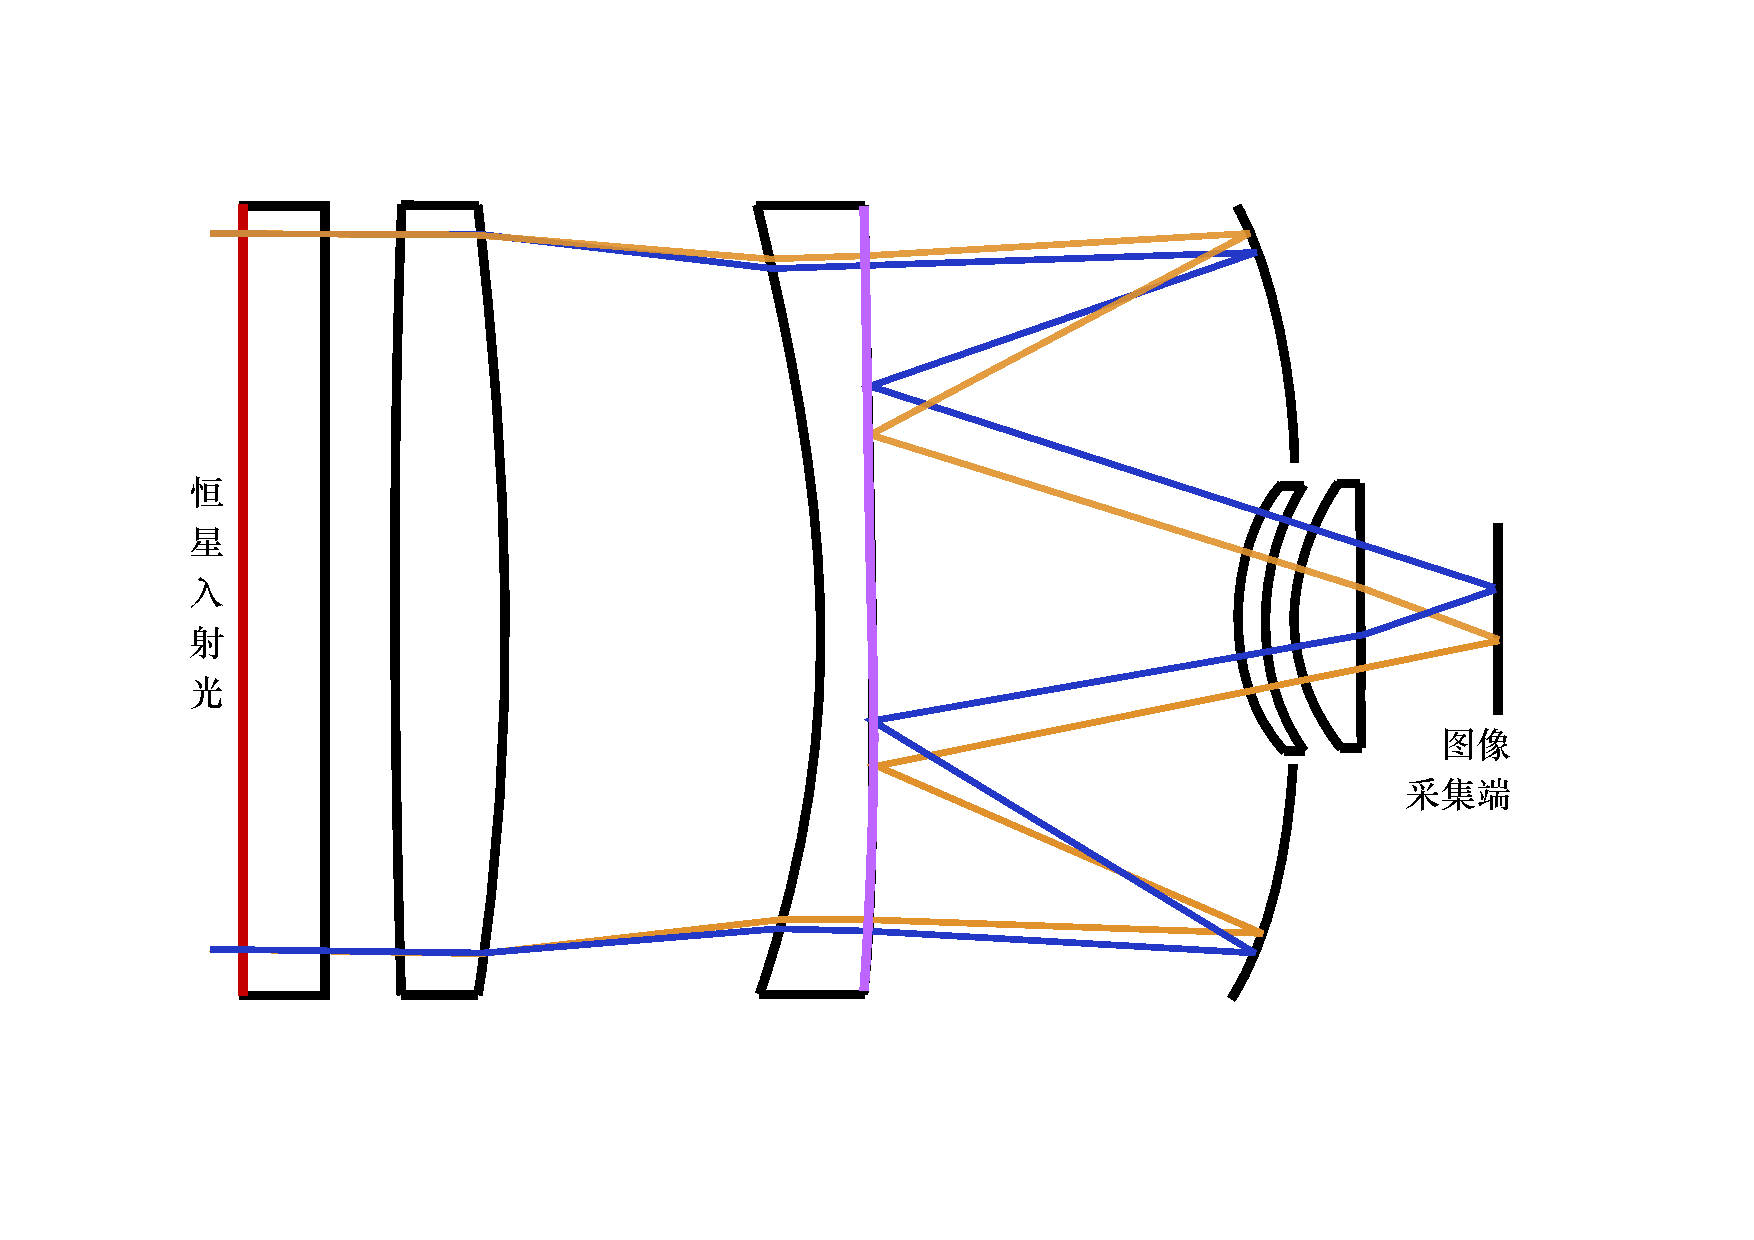
\includegraphics[width=1.0\textwidth]{figures/chapter2/f2_cstaroptics.pdf}
\caption[CSTAR 多镜面结构光路设计图。入射平板镜(最左侧)由改正镜与滤镜组成,最右侧的镜片为中空反射球面镜,中间子镜的右侧面涂有反射材料,该图与实际大小不成比例。]{CSTAR 多镜面结构光路设计图。入射平板镜(最左侧)由改正镜与滤镜组成,最右侧的镜片为中空反射球面镜,中间子镜的右侧面涂有反射材料。作图时未按照实际比例,参考自文献 \citen{ZhouX2010a}。}
\label{fig:cstaroptics}
\end{figure}

CSTAR 于 2008 年 1 月份,正式跟随南极科考队抵达冰穹 A 站点,可惜的是在第一个观测季度结束后,
望远镜只剩下 $i$ 波段镜面能正常观测。于是从 2008 年 3 月 4 日至 8 月 8 日(冰穹 A 站极夜),
CSTAR 共以 20 秒或 30 秒的曝光时间拍摄了超过 310, 000 张图片。多亏了极夜创造的连续不间断观测
条件,这些总曝光时间长达 1728 小时的图片数据表现出良好的科学状况与条件。

随着极昼的到来,科考人员取回了 CSTAR 的原始观测数据,国内两个小组分别开始了独立的分析工
作,国家天文台南极天文小组于 2010 年分别计算了台址当地 $i$ 波段的天光背景以及大气透明度
\cite{Zou2010},并释放出超过 10,000 颗恒星点源星表\cite{ZhouX2010b}。Wang 等人\cite{Wang2011}
则于来年在光变数据中找出了 157 颗变星(这高于该天区先前所知数量 6 倍)。随后 Wang 分别在随后
分别对测光给出大气消光、不均匀云层和周天效应的修正(文献 \citen{Wang2012,Wang2014})。

下面,本文将简要介绍文献 \citen{ZhouX2010b} 中主要的数据处理流程。在完成扣除本底和平场等预数据
处理后,Zhou 对每张原始图片采用了以 3,4 和 5 为半径的孔径测光(aperture photometry)。接着,
一张测光条件较好的图被选用作为标准参考,并用模式匹配来认证不同图内相同参考星的位置变化,并
同时矫正其他图片内点源的星等偏差量。以上操作得到标准星表后,其中 48 颗恒星被挑选出来和 
USNO-B1.0 参考星表对比从而得到最终星表。在以上的工作中,作者也发现数据中的鬼像修正对于进一步
提高测光精度有着非常重要的作用。

\subsection{鬼像简介以及修正 CSTAR 数据中的鬼像} \label{sec:ghost}

\subsubsection{鬼像以及 CSTAR 中的鬼像}
正如前文(\S \ref{sec:cstardesign})提到,鬼像在光学系统中并不算罕见,尤其是拥有大视场的施密
特望远镜。U.K. 施密特望远镜单元(UKSTU) 将鬼像的产生原因共归为五类,分别是乳化剂涂层、滤
片修正镜、改正镜、滤光片以及尖状鬼像。CSTAR 在设计上采取施密特卡式光学设计,因而鬼像很可
能产生于恒星入射光传播、折射与反射的过程中。UKSTU 手册\cite{1983ukstu} 将此类鬼像定性形容成
弥散状的斑点,且鬼像光斑坐标与产生鬼像的亮源位置关于光学轴对称。对于 CSTAR 而言,鬼像修正
十分必要,因为鬼像不仅会被误认证成一颗恒星源,还会叠加在背景恒星上从而造成额外的测光误差。

\begin{figure}[t]
\centering
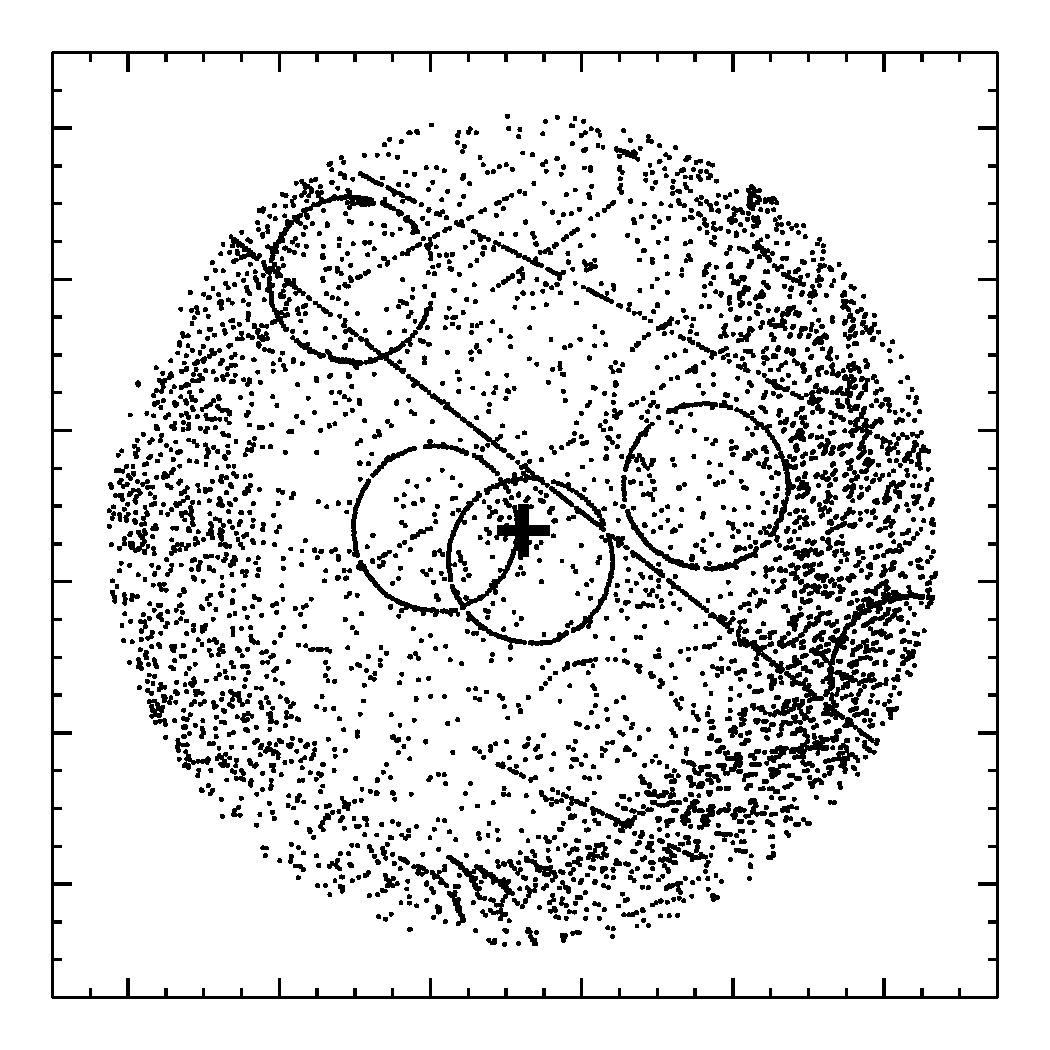
\includegraphics[width=1.0\textwidth]{figures/chapter2/f3_ghoststack.pdf}
\caption{周天鬼像叠加图,也即「脏」图。图中的圆弧结构为鬼像所致,黑色十字标注的是南极点。为了更好的看清鬼像的结构,我们已经将已确认的恒星从本图中剔除。视场边缘散点增多是因为畸变导致的模式低匹配效率,此外图中线状物为人造卫星。}
\label{fig:ghoststack}
\end{figure}

作为第一代南极天文望远镜,CSTAR 采取相对安全的凝视模式 --- 望远镜支撑点固定在冰层上,并
且对准南天极附近的天区观测。当恒星做周日运动时,星象斑也会在 CCD 上绕着南极点做近圆周运
动。若选取图「A5CH5029」作为标准参考图,那么经过恒星图案模式匹配(pattern match)后,其余
所有图相对于标准参考图的旋转角度便可被计算出。从而不同时间测得的图像内相同位置的恒星可被识
别认证。此时将相同恒星的本地坐标(pixel coordinate)通过旋转缩放等操作转化成标准参考图内的坐
标后,便可得到与其对应的主坐标(master coordinate)。从上一段文字中,已经得知鬼像(假恒星)
与产生鬼像的亮星关于光学轴对称,所以当恒星们时时刻刻被匹配上的同时,鬼像却只能经过一个周天
后才能匹配上自己。若把一天之内所有拍摄的图片作叠加,然后将同一颗恒星给抹去后,我们可得到周
天鬼像叠加图(请查阅图 \ref{fig:ghoststack})。从图中可以看出,鬼像的转动方向与周日运动方向相
反,鬼像因此也很可能周期性地「撞」到恒星。当然,如果将南极冰川板块的微弱移动\cite{ZhouX2013}
与恒星自身的运动考虑在内,鬼像很有可能在一天内遭遇到多颗恒星,从而对恒星亮度造成多达约 1.0 
星等的变化(如图 \ref{fig:lcwghost} 与图 \ref{fig:ghostseq})。若不仔细地处理这种变化则很可能被误认为恒
星自身的性质,例如恒星耀斑\cite{Liang2016},因此修正鬼像是后续天体物理研究,如搜寻系外行星
\cite{Wang2014CSTAR} 以及变星\cite{Yang2015}等等的前期基础工作。

\begin{figure}[t]
\centering
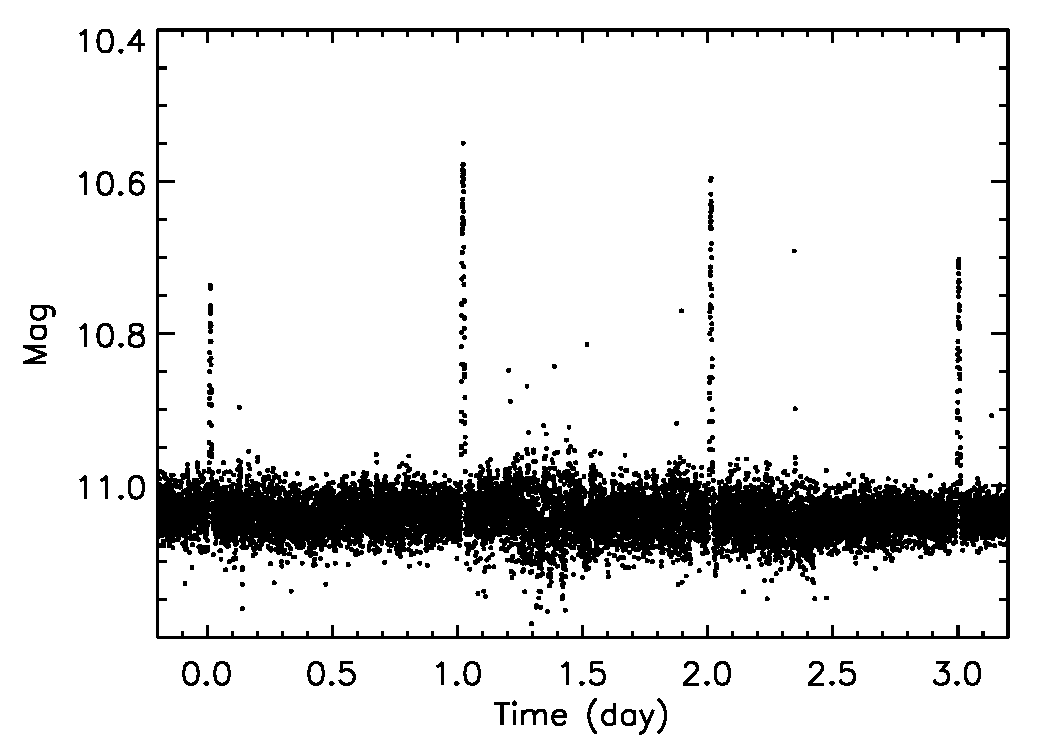
\includegraphics[width=1.0\textwidth, trim={0.0cm 0.5cm 0 0}]{figures/chapter2/f4_lcwghost.pdf}
\caption{CSTAR 视场内坐标为 R.A.: $23^\tif{h}24^\tif{m}28.4^\tif{s}$,Decl.: $-89^{\circ}25'10.6''$ 恒星的光变曲线。通常特定的鬼像会在一个恒星日内遭遇该被影响的恒星一次,从而将恒星的亮度提高半个星等。}
\label{fig:lcwghost}
\end{figure}

\begin{sidewaysfigure}
\centering
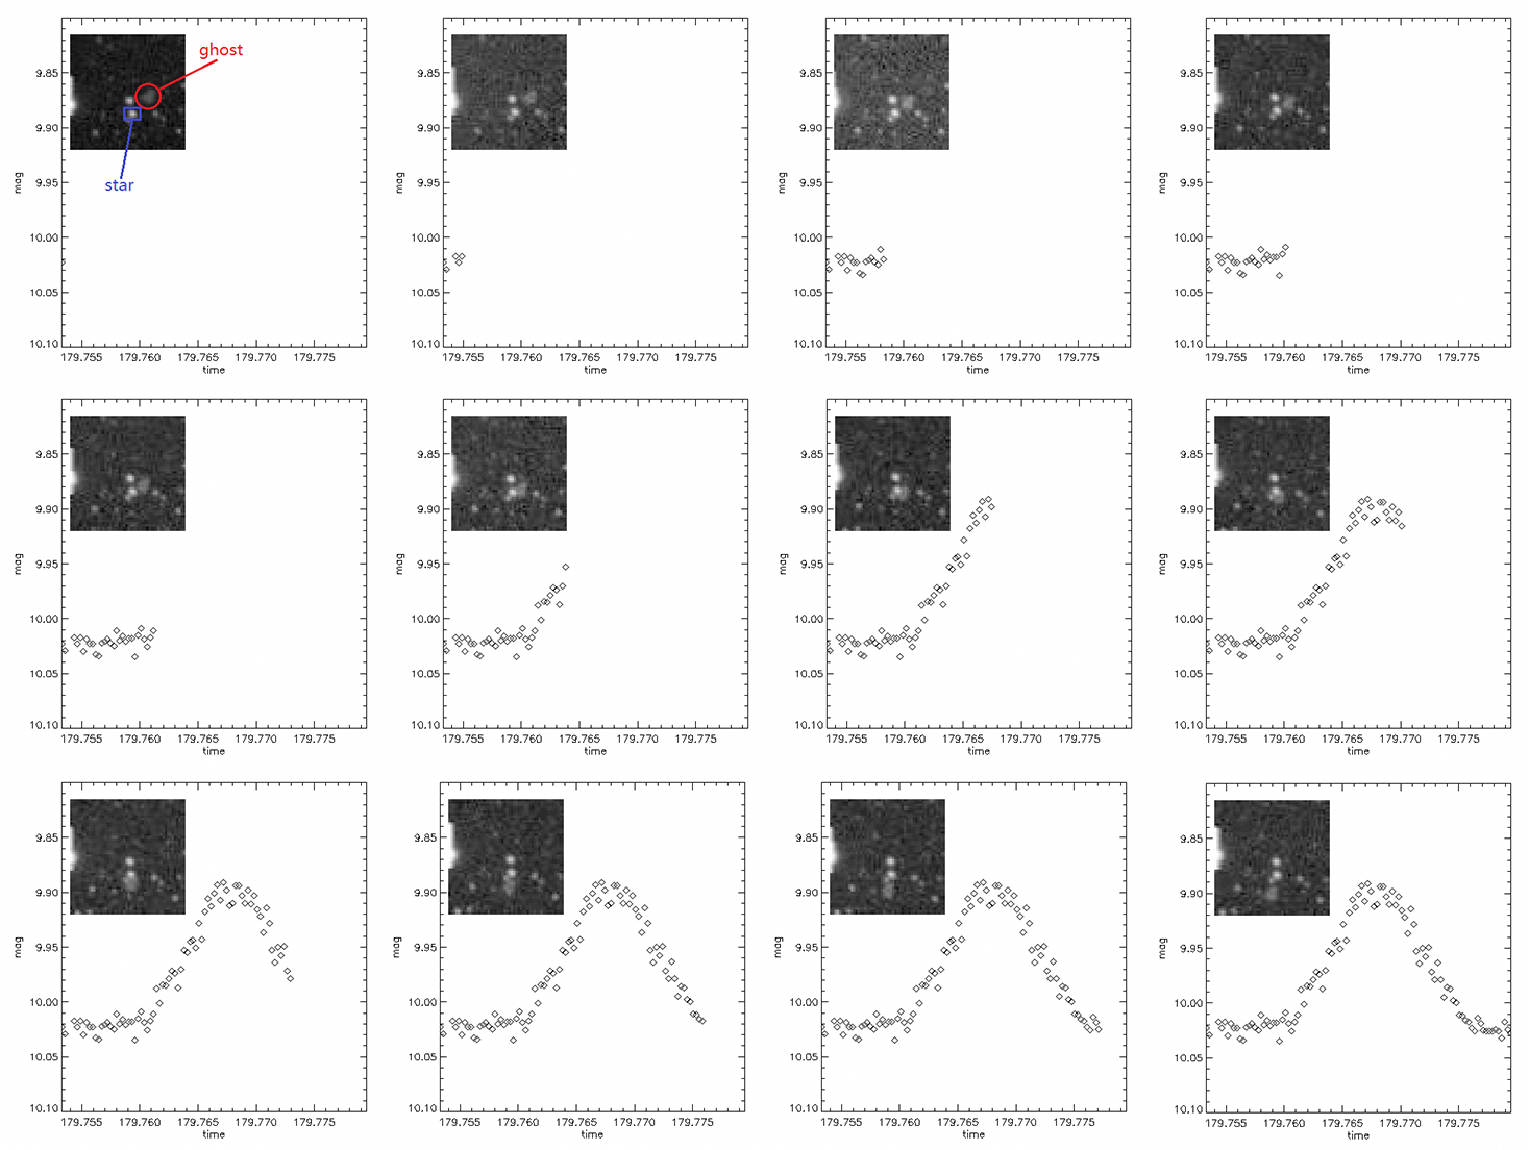
\includegraphics[scale=0.8]{figures/chapter2/f5_ghostseq.pdf}
\caption[坐标相对固定的恒星(绿色标志)遇到鬼像(红色标注的模糊状弥散源)前后,恒星星等的变化程度原始图片数据示意。]{坐标相对固定的恒星(绿色标志)遇到鬼像(红色标注的模糊状弥散源)前后,恒星星等的变化程度原始图片数据示意。每张快照的纵坐标为星等值,横坐标为时间,如需查看此图清晰的动画版本请前往网址 \url{https://github.com/meldonization/PhD_Dissertation/blob/master/figures/chapter2/ghost_animation.gif}。}
\label{fig:ghostseq}
\end{sidewaysfigure}


\subsubsection{CSTAR 鬼像修正方法}

为了扣除所有被影响的恒星流量中鬼像的污染,我们首先得确认产生这些鬼像的前身,即视场中的亮源。
之所以采取此途径是因为鬼像通常为暗弱的延展源,背景噪声对它们的孔径测光影响很大,直接扣除
被影响恒星中鬼像的孔径测光流量的做法会变得非常不可靠。找到产生鬼像的亮源后,我们会将被被影响
恒星的星等变化程度极短出来,最后就可以对 CSTAR 的数据进行系统性的修正。

我们因此发展了一整套识别、处理、计算并消除鬼像对恒星星等	影响的流程。具体如下:

\begin{enumerate}[leftmargin=1\parindent]

\item \textbf{确定光学系统对称轴和产生鬼像的亮源。} CSTAR 视场较大,点源密集,因而对每个鬼像
每张图做修正几乎是不可能完成的任务,这里我们只查找星场中最显著的鬼像环。此种考虑也是由于望
远镜观测的极限星等限制,因而只有最亮的恒星才会产生鬼像。当我们将星表中的前 100 颗亮星与最明
显的鬼像环圆心做位置匹配,那么成功被匹配的亮星也就是产生鬼像的源。一旦产生鬼像的源被确定后,
我们便可将鬼像的主坐标 [$X$, $Y$] 转换成每张图片中的本地坐标 [$x$, $y$]。通过交叉联立此本地坐
标和上文提到的亮星坐标,可以进一步得到望远镜系统的光学对称轴在 CCD 上的像素坐标值。

\item \textbf{定量的描述鬼像对背景星的影响。} 在知晓系统的光学对称轴后,我们可以从文献 
\citen{Wang2012} 中找到产生鬼像的恒星、鬼像以及被鬼像影响恒星的星等数值,且这三者中最后一个
物理量会随着鬼像和恒星之间的距离变化而发生改变。下文统一用 $d$ 替代鬼像中心与被鬼像影响恒星
中心之间的距离,用 $m_\tif{g},\,m_\tif{gs},\,m_\tif{s}^0$ 和 $m_\tif{s}^1$ 分别表示鬼像的星等、鬼像源
亮星的星等、被鬼像影响前后背景星的星等。本文采取两个基本假设:一、鬼像源亮星流量与鬼像流量的
转化率为 $f_0$,即 $F_{\rm{g}}=f_0\cdot F_{\rm{gs}}$;二、鬼像对背景星造成的光子数影响比例 $f_1 $ 
只是距离 $d$ 的函数,$\Delta F_{\tif{s}}=F_{\tif{s}}^1-F_{\tif{s}}^0=f_1(d)\cdot F_{\tif{g}}$。若此时带入
流量与星等之间的转换关系 $m=-2.5\lg F+m_0$,我们可以得到如下两个等式:


\begin{equation} \label{eq:ghostformular}
\arraycolsep=1.2pt\def\arraystretch{1.3}
\left\{
\begin{array}{l}
m_{\tif{g}} = -2.5 \lg f_0 + m_{\tif{gs}} \\
f_1(d) \cdot f_0 \cdot C^{m_{\tif{gs}}} = C^{m^1_{\tif{s}}}-C^{m^0_{\tif{s}}}  \, \ ,
\end{array} 
\right. 
\end{equation} \myequation{修正鬼像星等差的基本公式}
其中常数 $C=\lg 2.5$。从统计上,我们可从鬼像、源恒星以及被影响的背景星的列表中拟合两个自由参
数 $f_0$ 和 $f_1(d)$。这里需要指出的是不同亮星产生的鬼像之间的参数并不完全一致,为了方便起
见,我们归一化处理了第二个参数 $f_1(d)$。

\item \textbf{修正星表中的鬼像影响。} 以上两步完成后,我们可估算每张图内的未知参数 $f_0$ 和 $f_1(d)$。假设图片拍摄时间为 $t$,那么在带入每张图内每个恒星的修正量后,可得到去除鬼像污染的新光变曲线序列 $(t, d, mag_{\tif{s}}, mag_{\tif{gs}})$以及全新的星表。

\end{enumerate}

\begin{table}[t]
\centering
\caption{CSTAR 星表中主要产生鬼像的亮星列表。} 
\label{tbl:ghostsource}
\begin{tabular}{cccccc}%{1.0\linewidth}{@{\extracolsep{\fill}}ccccccc}
\hline \hline
CSTAR ID	&    R.A.   &   Decl.  	       &    masterX    &   masterY    &    $i$          \\ 
	        	&  (h:m:s) & (d:m:s) 	       &      (pixel)      &     (pixel)      &  (mag)       \\ \hline
00003   	& 49:03.3 & -88:16:34.99 & 7497.2864   & 1386.2566   & 6.1357  	\\
00004   	& 15:58.6 & -87:33:53.25 & 1350.1814   & 8661.678     & 6.1444  	\\
00006   	& 34:34.0 & -89:46:18.97 & 5129.6065   & 5103.6644   & 6.3055  	\\
00007  	& 08:26.2 & -88:57:34.07 & 2812.204     & 4118.1307   & 6.3671  	\\
00008   	& 15:55.2 & -87:58:09.94 & 1740.2338   & 1388.6649   & 6.4489  	\\
00009   	& 42:07.6 & -89:27:37.16 & 6386.3986   & 4679.7432   & 6.4995  	\\
00011  	& 20:07.4 & -88:14:48.27 & 8033.5867   & 7374.1179   & 6.5395  	\\
00012  	& 39:55.7 & -88:39:19.55 & 4151.218     & 7494.304     & 6.5944  	\\
00018  	& 45:45.4 & -88:48:57.98 & 2940.9191   & 3000.1653   & 6.8181  	\\
\hline \hline
\end{tabular}
\end{table}

\subsubsection{鬼像修正结果及讨论}

当拟合鬼像环半径数值(约 107 像素大小)、圆心位置坐标,并通过 match 程序
\footnote{源代码链接 \url{http://spiff.rit.edu/match/}}和文献 \citen{Wang2012} 给出的参考新表对比后,
我们得到了一批产生鬼像的恒星列表(表格 \ref{tbl:ghostsource})。由图 \ref{fig:starwghost} 可知鬼像
与源恒星 $i$ 波段的星等差约为 5.5,考虑到 CSTAR $i$ 波段的极限星等约为 14 等,因而在接下来计算
背景恒星星等受影响量的过程中,我们仅需考虑 $i < 8.5$ 的亮星产生的鬼像。

\begin{figure}[h!]
\centering
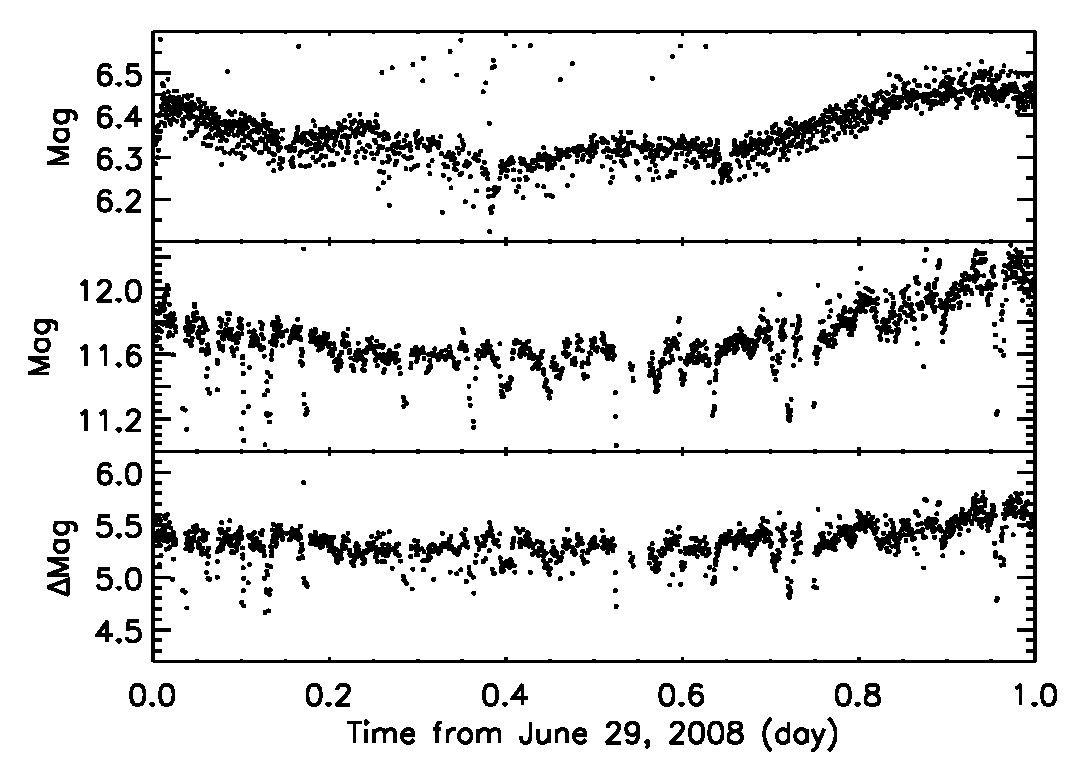
\includegraphics[width=0.92\textwidth, trim={0.3cm 0.5cm 0 0}]{figures/chapter2/f6_starwghost.eps}
\caption{上栏为产生鬼像的源恒星(R.A.: $21^\tif{h}08^\tif{m}44.2^\tif{s}$,Decl.: $-88^{\circ}57'21.6''$)在一天内的星等变化图;中间栏为该源对应鬼像在这天内的星等变化;下栏为两者星等的差量。}
\label{fig:starwghost}
\end{figure}

\begin{figure}[h!]
\centering
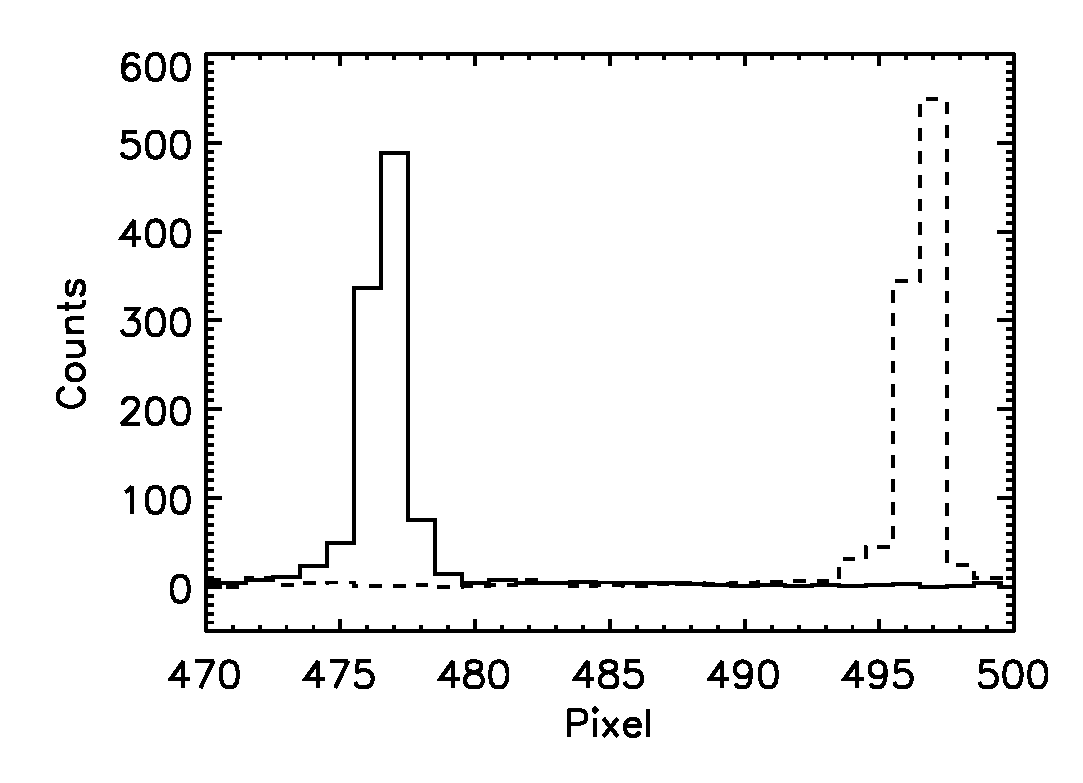
\includegraphics[width=0.92\textwidth,trim={0.5cm 0.5cm 0 0}]{figures/chapter2/f7_opticaxispix.eps}
\caption{光学对称轴在 CCD 上像素坐标的统计直方图,直方图格点宽度为一个像素点。图中实线为本地 $x$ 坐标像素值,虚线则为 $y$ 坐标。}
\label{fig:opticaxispix}
\end{figure}

然而在实际情况中,并不是所有星等量过 8.5 的恒星均会产生鬼像。亮星产生鬼像有很多条件,最重要
的两个因素是这些亮源距离视场中心以及光学对称轴的距离。原理上讲,当亮星距离视场中心或者对称
轴中心太远,它在镜面反射层之间被反射的光需要经过更长的光学路径来传播,产生的鬼像也因此而更
暗弱。


\begin{figure}[t]
\centering
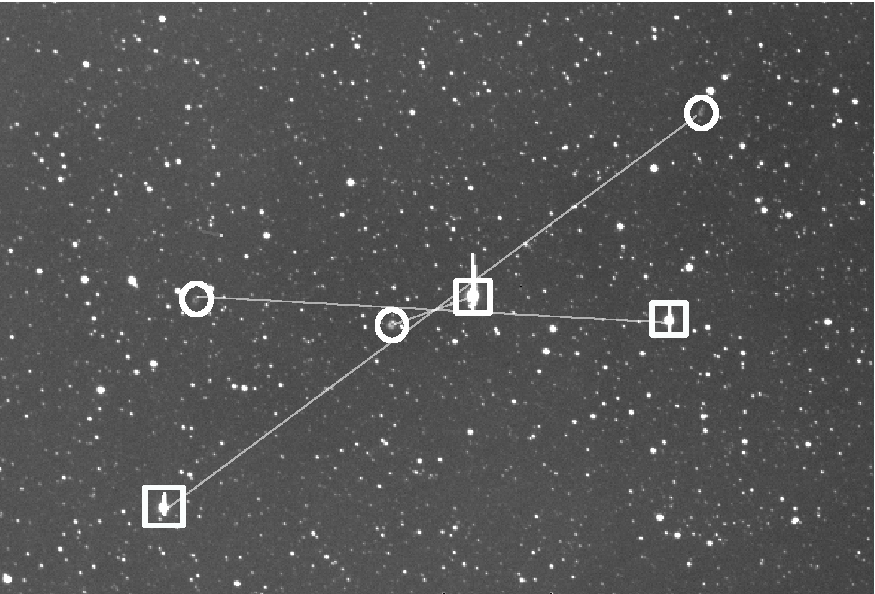
\includegraphics[width=0.95\textwidth]{figures/chapter2/f8_opticaxisimg.pdf}
\caption{选定的图片文件名为「16RE0312.fit」中光学对称轴示意图。方框选中的亮源(拥有光子溢出竖线)与圆环内的弥散鬼像相交于同一个像素点,即光学对称点(轴)。}
\label{fig:opticaxisimg}
\end{figure}

在得到鬼像源亮星列表后,我们将该列表和鬼像环内的所有恒星做比较。这样做可以得到每张图中真正
的鬼像和 CSTAR 系统的光学对称轴在 CCD 上的像素坐标。如图 \ref{fig:opticaxispix} 所示,光学对称
轴的本地坐标为 $[477\pm2,\ 297\pm2]$。该值也同样经过真实图像的测试(图 \ref{fig:opticaxisimg})。
考虑到鬼像以及其对应产生亮源之间的几何构造,不难得到鬼像环半径与光学对称轴和南极点之间距离
的关系式:
\begin{equation} \label{eq:ghostgeometry}
r_{\tif{ghost}}=2\cdot d_{\tif{Pole, axis}} \ \ . 
\end{equation} \myequation{鬼像半径与南极点以及光学对称轴之间的几何关系}

如果将南极点的本地坐标值(即 $[523,\,467]$)与上文提到的光学对称轴坐标值(即 $[477,\ 497]$)带入上式,可算得鬼像的半径理论值为 109 像素,这也和前面的拟合值一致。

\begin{figure}[ht!]
\centering
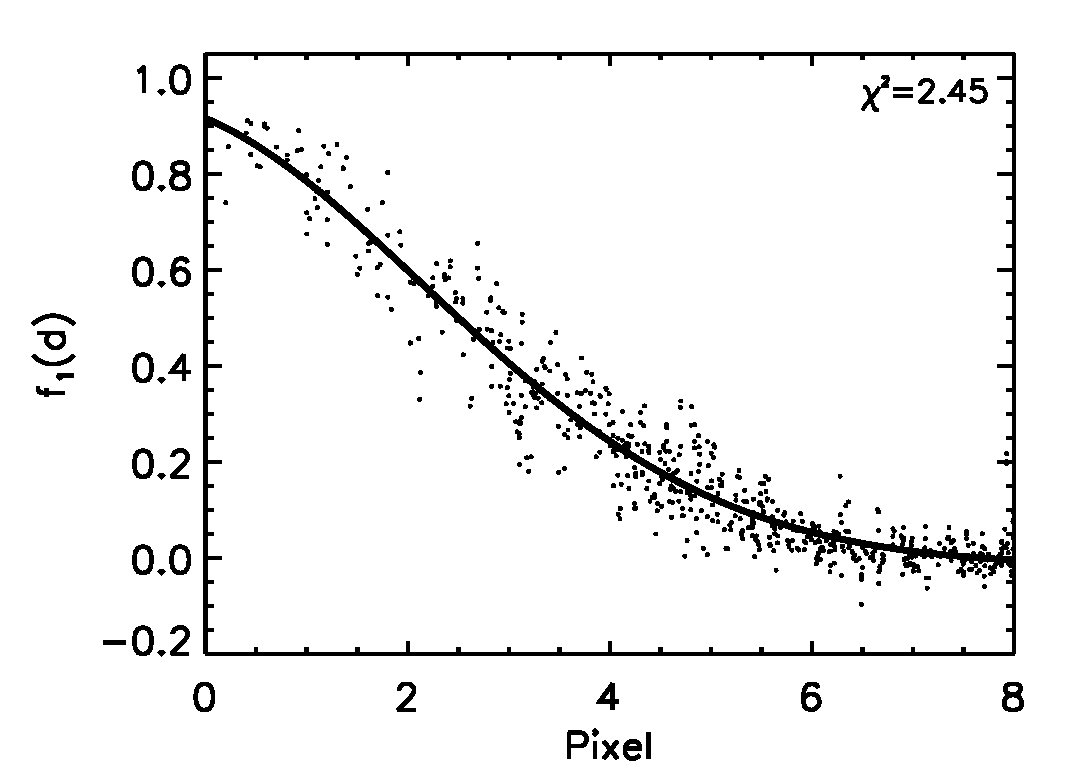
\includegraphics[width=0.8\textwidth, trim={0.5cm 0.3cm 0.5cm 0}]{figures/chapter2/f9_ghostfit.eps}
\caption{鬼像影响因子 $f_1(d)$ 与被影响背景恒星和鬼像之间距离的依赖关系。实线为形式如方程 \ref{eq:ghostf1d} 的拟合曲线,当两者之间的距离大于约 6 个像素时,鬼像几乎不对该星的亮度造成影响。相反,当鬼像完全重叠在背景恒星上时,鬼像自身高达 97\% 的光子流量都会被算入恒星的孔径测光亮度中。}
\label{fig:ghostfit}
\end{figure}

\begin{figure}[ht!]
\centering
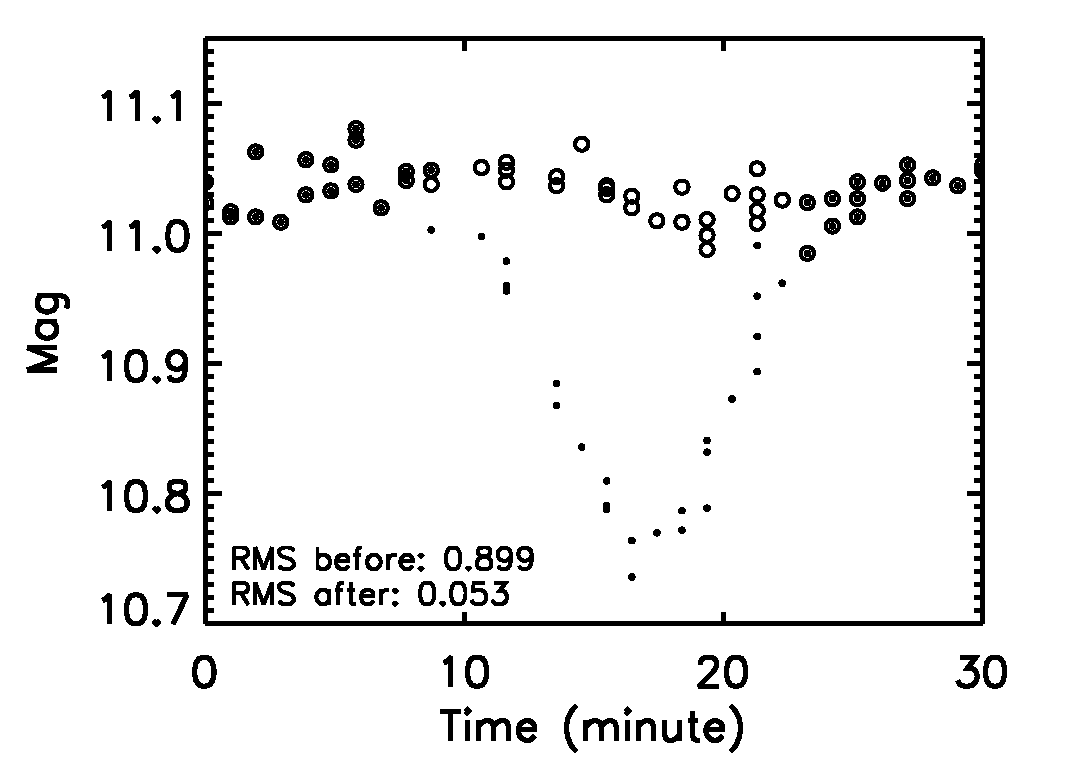
\includegraphics[width=0.8\textwidth, trim={0.5cm 0.3cm 0.5cm 0}]{figures/chapter2/f10_deghost.eps}
\caption{鬼像修正前后(分别为点和圆)恒星的光变曲线。此恒星坐标为 R.A.: $23^\tif{h}24^\tif{m}28.4^\tif{s}$,Decl.: $-89^{\circ}25'10.6''$。当鬼像距离恒星达到 6 个像素点的临界值后,鬼像修正程序便会自动在恒星的光变曲线基础上计算影响值并做修正。如图所示,此方法可以大幅度减小恒星光变曲线的弥散误差。}
\label{fig:deghost}
\end{figure}


至于第一个影响因子 $f_0$,图 \ref{fig:starwghost} 已经展示了鬼像与亮星之间的亮度变化基本趋于一
致,这个差别值大概为 5.4 星等,即对应亮星 0.7\% 的光子流量被反射再聚集成鬼像。但与此同时,
我们应该意识到实际中的鬼像更加复杂:不同的位置、星等都会给 $f_0$ 因子带来不确定性。

如此一来,在计算第二影响因子的过程中,我们一律假设 $f_0 =  0.7\% $。在对星象班等天文观测数据
中,自然的假设便是此函数为高斯函数。因为鬼像与恒星之间的距离减小到临界值时,恒
星的亮度才开始被影响,而这个临界值就是鬼像展源半径的大小。上述高斯函数具有如下形式:
\begin{equation} \label{eq:ghostf1d}
f_1(d) \simeq A_0 \cdot e^{-Z^2/2} \ \ , 
\end{equation} \myequation{鬼像影响因子参数 $f_1(d)$}
其中 $Z = (d-A_1)/A_2,\ A_0 \approx 0.97,\ A_1 \approx -0.86$,$A_2 \approx 2.99$。这边需要强调的
是由于并不知道背景星被鬼像遮挡后的真正星等值,因而我们假设星等值为固定值(取自文献 
\citen{Wang2012})。上述高斯函数也正好说明鬼像的典型半径为 6 个像素点,这明显大于孔径测光所
选取的孔径大小\cite{ZhouX2010b},这也从侧面说明了利用孔径测光直接求鬼像星等来修正星表的做法
在此处并不适用(如图 \ref{fig:ghostfit} 所示)。

最后一步,我们需要将表达式 \ref{eq:ghostf1d} 中的关系带入每张图中,并对在鬼像和任意恒星靠近时
修正对应的鬼像流量值即可得到无鬼像版本的星表数据\footnote{星表文件请访问网址 \url{http://explore.china-vo.org/data/cstar/f}}。前文中给出的例子表明本文的鬼像修正是真实且有效的,当然也还有部分误差来源无法还原,比如 $f_0$ 因子的不确定性,以及最初的星表位置精度可能并不能达到 2 个像素半径。

包括鬼像修正在内的各种预数据处理工作都对提高测光精度有着极为重要的作用。修正鬼像并提高精度
后的数据有利于研究耀斑、变星以及系外行星搜寻\cite{Liang2016,Yang2015,Wang2014CSTAR}。另外对于今后的巡天工作,例如为下文提到的 AST3 望远镜做出铺垫\cite{Cui2008}。


\section{AST3-2 项目中系外行星的巡天策略} \label{sec:ast3}

在天文学研究中,观测是最基础也是最重要的环节。科学项目中,观测台址,选源以及策略直接决定了
预定科学价值的实现程度,天穹 A 台址的优势之处我们从前文也已经有大概了解。紧随着 CSTAR 项目,
AST3 望远镜同样为一个大视场广角巡天项目。大视场优势就在于望远镜能够同时利用多波段检测一大片
天区,本来相对低效的巡天项目可以有许多丰富的科学成果(如利用凌星法探测系外行星)。AST3 顾
名思义,由三个 50/68 cm 的修正施密特望远镜组成。后端装备的是 10k $\times$ 10k 的 的帧转移 CCD 
相机。其中第一台 AST3-1 于 2012 年 3 月正式安装就位并投入使用。但不幸的是该台望远镜于当年 5 月
份停止工作。一批关于变源搜索的成果也已经浮现,如文献 \citen{Li2015,Wang2017}。

而经过两年多的测试,AST3-2 也于 2015 年正式着陆南极领土并投入工作。图 \ref{fig:ast3tele} 为前
两台 AST3 望远镜在南极冰穹 A 站点的合影。系外行星搜索作为本次观测的科学目标之一,也因此而得到 
2016 极夜一个多月的观测时间。下面将主要介绍 AST3-2 望远镜的观测策略(strategy and 
pipeline)。整个脚本自动化观测的流程(如图 \ref{fig:ast3obs})包括初始化输入、自动观测、报错系统
以及预数据处理四个主要环节:


\begin{figure}[t]
\centering
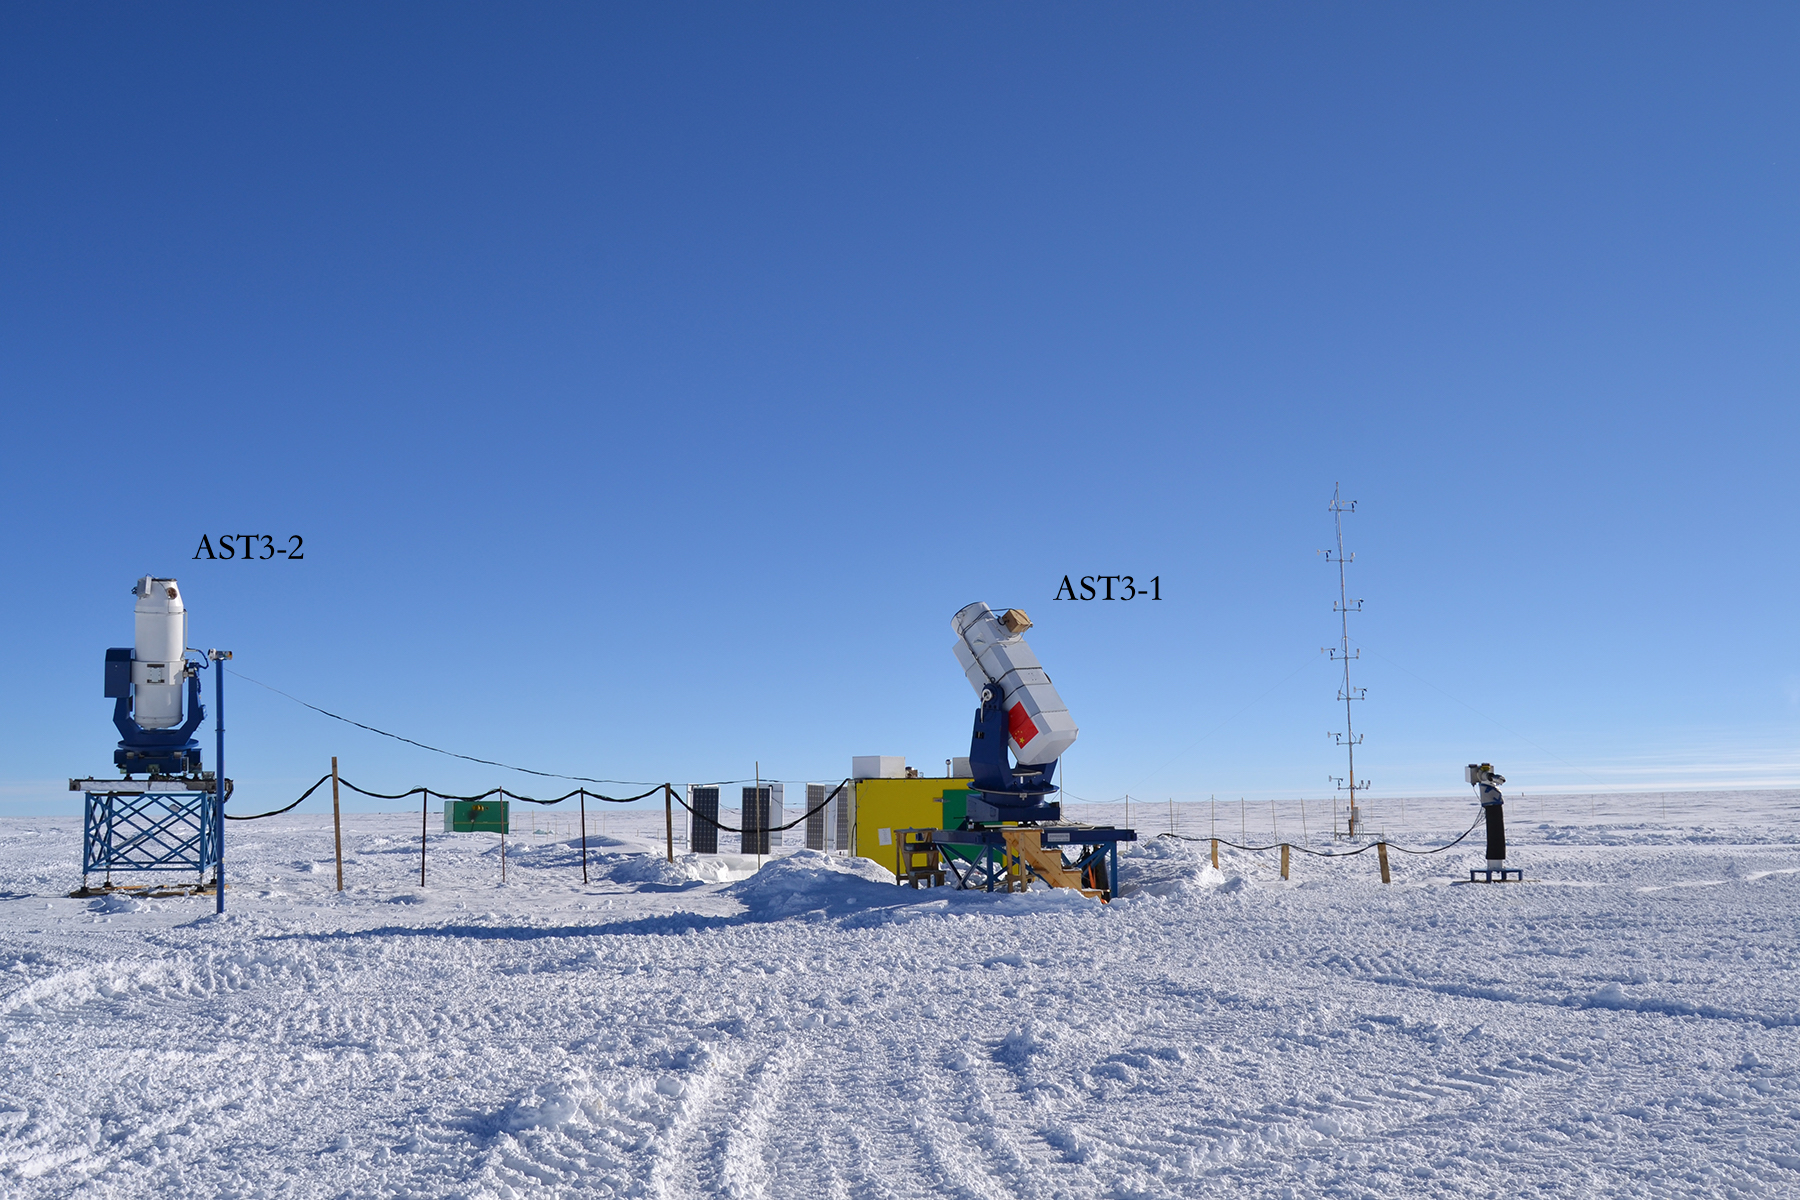
\includegraphics[width=1.0\textwidth]{figures/chapter2/f11_ast3.jpg}
\caption{AST3-2望远镜(左侧)就位于南极天穹 A 观测站。本图拍摄者为天文科考科考人员杜福嘉。}
\label{fig:ast3tele}
\end{figure}

\begin{enumerate}[leftmargin=1\parindent] 

\item[--] \textbf{初始化输入} {} 整个观测自动化程序从这里开始。首先观测开始会生成当天的
日志记录。紧接着读取输入参数并检查文件系统是否正常。如果正常则读取我们的目标观测天区信息文
件,跳转到下一步自动观测流程。


\item[--] \textbf{观测操作} {} 因为 AST3 有了一整套的望远镜跟踪系统,因而观测操作除了正
常的 CCD 曝光采集恒星图像文件以外,还额外需要控制望远镜的正常指向和信息反馈。特别是对与风雪
恶劣的天气,需要额外小心操作并及时采集错误。


\item[--] \textbf{数据处理} {} 为了实时检测系统的工作状况,除了有一套实时摄像头对准 
AST3之外\footnote{远程实时检测网址\url{http://aag.bao.ac.cn/klaws/}。},我们还额外加入了远程定位
(astrometry)与测光(photometry)模块。这部分环节和观测模块
各自独立运行,可返回非常实用的实时消光以及望远镜指向跟踪精度等信息。


\item[--] \textbf{报错系统} {} 容错子系统是观测策略中必不可少的成分。以上描述的各个流程都会对错误守护进程实时反馈,一旦有错误报错系统会在当前操作结束后中断观测并向远程(如南京大学天文与空间科学学院远程观测实验室本地终端)传送错误信息。本地系统抓取到错误后也会立即通过邮件系统通知相关人员。

\end{enumerate}

\begin{figure}[t]
\centering
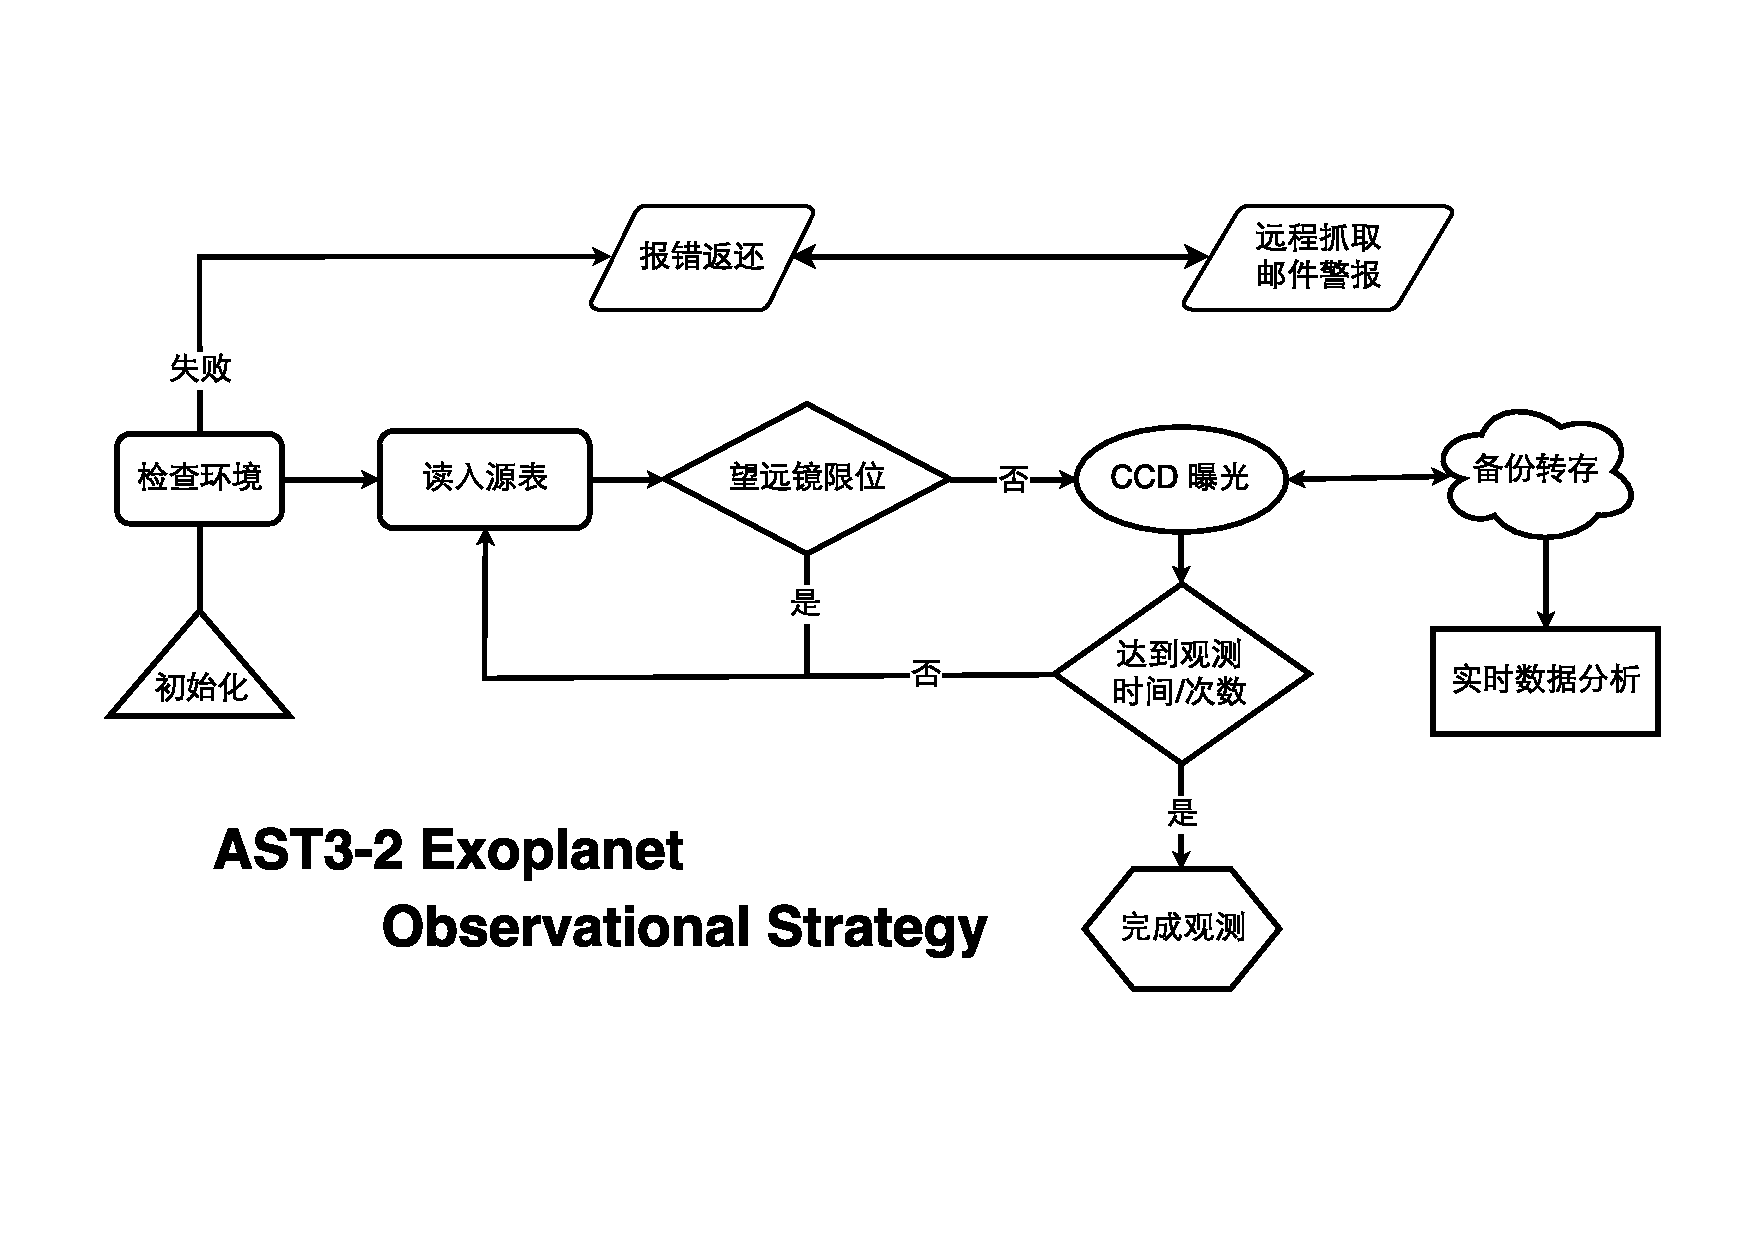
\includegraphics[width=1.0\textwidth]{figures/chapter2/f12_ast3pipeline.pdf}
\caption{AST3-2 观测策略。整体流程包括初始化输入,观测,容错以及数据处理共四个环节。}
\label{fig:ast3obs}
\end{figure}

充分完善以上流程\footnote{源代码链接 \url{https://github.com/meldonization/exoSurvey}。}对于保证观测(尤其是极地环境连续黑夜)非常重要,尤其是在 \S \ref{sec:pexample} 提到的极短周期行星探测以及性质刻画(Zhang et al. in prep.)。经过以上的充分实验,我们也完全有理由相信,随着今年科考人员采集数据归来,一批新的科学成果即将涌现。现有的包括 CSTAR 和 AST3 在天穹 A 台址的天文望远镜必定能助力今后即将诞生的昆仑暗宇宙巡天望远镜(KDUST),前人的观测以及数据处理也会一同作为试金石,铺助南极科学日益精进。


